
\documentclass[10pt,twocolumn]{witseiepaper}
%
% All KJN's macros and goodies (some shameless borrowing from SPL)
\usepackage{KJN}
\usepackage[super]{nth}
\usepackage{subcaption}
\usepackage{listings}
\usepackage{amsmath}
\usepackage{epstopdf}
\usepackage{xcolor}
\usepackage{textcomp}
\usepackage{listings}
\usepackage{alltt}
%\usepackage{matlab-prettifier}
\usepackage{graphicx}
\usepackage{changes}
\usepackage{makecell}
\usepackage{verbatim}
\usepackage{algorithm,algpseudocode}
\usepackage{balance}
\usepackage{pdfpages}
\usepackage{makecell}
\usepackage{color} %red, green, blue, yellow, cyan, magenta, black, white
\definecolor{mygreen}{RGB}{28,172,0} % color values Red, Green, Blue
\definecolor{mylilas}{RGB}{170,55,241}
%\usepackage{flafter}

%\usepackage[parfill]{parskip}
%\usepackage{titlesec}
%
%\titleformat{\subsubsection}
%{\normalfont\normalsize\itshape}{\thesubsubsection}{1em}{}
%\titlespacing*{\subsubsection}{0pt}{3.25ex plus 1ex minus .2ex}{0ex plus .2ex}

\lstset{language=Matlab, % Set colour for matlab code
	breaklines=true,%
	morekeywords={matlab2tikz},
	keywordstyle=\color{blue},%
	morekeywords=[2]{1}, keywordstyle=[2]{\color{black}},
	identifierstyle=\color{black},%
	stringstyle=\color{mylilas},
	commentstyle=\color{mygreen},%
	showstringspaces=false,%without this there will be a symbol in the places where there is a space
	numbers=left,%
	numberstyle={\tiny \color{black}},% size of the numbers
	numbersep=9pt, % this defines how far the numbers are from the text
	emph=[1]{for,end,break},emphstyle=[1]\color{red}, %some words to emphasise
	%emph=[2]{word1,word2}, emphstyle=[2]{style},    
}
%
% PDF Info
%
\ifpdf
\pdfinfo{
/Title (INSTRUCTIONS AND STYLE GUIDELINES FOR THE PREPARATION OF FINAL YEAR LABORATORY PROJECT PAPERS : 2005 VERSION)
/Author (Ken J Nixon)
/CreationDate (D:200309251200)
/ModDate (D:200510121530)
/Subject (ELEN417/455 Paper Format, 2005)
/Keywords (ELEN417, ELEN455, paper, instructions, style guidelines, laboratory project)
}
\fi

%%%%%%%%%%%%%%%%%%%%%%%%%%%%%%%%%%%%%%%%%%%%%%%%%%%%%%%%%%%%%%%%%%%%%%%%%%%%%%%
\begin{document}


\title{TITLE}

\author{Sasha Berkowitz (818737) \& Lara Timm (704157)
\thanks{School of Electrical \& Information Engineering, University of the
Witwatersrand, Private Bag 3, 2050, Johannesburg, South Africa}
}


%%%%%%%%%%%%%%%%%%%%%%%%%%%%%%%%%%%%%%%%%%%%%%%%%%%%%%%%%%%%%%%%%%%%%%%%%%%%%%%
%
\abstract{}

\keywords{}

\maketitle
%\thispagestyle{empty}
\pagestyle{plain}
\setcounter{page}{1}


%%%%%%%%%%%%%%%%%%%%%%%%%%%%%%%%%%%%%%%%%%%%%%%%%%%%%%%%%%%%%%%%%%%%%%%%%%%%%%%
\section{INTRODUCTION}

File Transfer Protocol (FTP) is a protocol used  to transfer files between two hosts over a TCP or IP network~\cite{FTPbeginners}. In it's operation FTP makes use of two TCP connections, a control connection and a data connection. The control connection, used to send control information, is opened and remains open throughout the duration of the user session~\cite{topDownApproach6th}. The data connection is non-persistent; a new data connection is established for each new file transfer~\cite{topDownApproach6th}. The main objectives of FTP include the promotion of file sharing, to encourage the use of remote computers, to shield users from variations in file storage systems among hosts and to ensure reliable and efficient data transfer~\cite{rfc959}. 

%Using the python programming language as well as basic socket methods, a File Transfer Application is designed and tested. Additionally, a basic FTP User Interface (UI) is developed to interact with the remote FTP server in an intuitive way.

Detailed within the sections below are a overview of the implemented system and its command/reply messaging exchange, a working description of the system and code base, the results of system testing and a critical analysis thereof. Also included is the division of work between the project partners.

%%%%%%%%%%%%%%%%%%%%%%%%%%%%%%%%%%%%%%%%%%%%%%%%%%%%%%%%%%%%%%%%%%%%%%%%%%%%%%%
\section{SYSTEM DESCRIPTION} 

An FTP client and server pair has been designed and implemented as per RFC~959 specifications~\cite{rfc959}. By implementing the system in such a way, both the server and client are compatible with standardised servers and clients. The system is designed and tested on the  Windows OS.

\subsection{FTP Server}

The FTP server is hosted locally, and can be accessed by an FTP client which is either connecting from the hosts computer, or from a computer running on the same Local Area Network (LAN) via the server's IP address. 

To provide unique user experience, the server maintains a user repository, within the servers local file system, for each registered client. To gain access to their remote repository, the user must be successfully authenticated using their unique username and password. Clients trying to connect without a registered username and password are not permitted to access the server file system.

The server is implemented in accordance with the RFC~959 specification. The implemented features of the system go beyond those of the minimum requirements set out by the standard, improving the system's general functionality and usability. 

To allow for more than one client to be connected to the server at a time, the server program is multithreaded. Each new client connection is handled by a separate thread, and up to five simultaneous connections can be established by FTP clients. 

To communicate file, system and transfer status to the client, the server makes use of a number of RFC~959 specified reply codes. These codes enable the client to detect errors and react accordingly. Further discussion of the FTP command and replies can be found in Section~\ref{sec:command/reply}

\vspace*{-2mm}
\subsubsection*{Unimplemented features: }
In accordance with the RFC~959 minimum requirements, the default file structure and transfer mode for exchange should be implemented. Functionality for \textit{record} and \textit{page} structures, as well as for \textit{block} and \textit{compressed} transfer modes were not implemented. The project group deemed theses features unnecessary as file transfer is still possible in their absence.

\subsection{FTP Client}

The FTP client is composed of two working parts, a Graphical User Interface (GUI) and a logical FTP client. The user interacts with the GUI which instructs the FTP client to interact with the FTP server. In this way the interface is separated from the logic layer, following the separation of concerns principle.

\vspace*{-2mm}
\subsubsection{Client Logic} $     $

The FTP client is hosted locally and can connect to a server hosted either locally (on the client's computer) or over a LAN connection. To connect to the server, the client must know the IP address and port on which the server is listening for a TCP connection.

The responsibility of the logical FTP client is to interact with the server in accordance with FTP standards. The client translates raw data received from the GUI and formats it to comply with the RFC~959 specification. In this way, the client can not only interact with the designed server, but also  with a range of standard FTP servers.

It is the responsibility of the client to handle errors that are not relevant to the server. Such errors include trying to upload a file that does not exist in the clients file system and handling errors to do with incorrect formatting of client commands.

\vspace*{-2mm}
\subsubsection{Client Interface} $      $\label{GUI}

%Sash%%%%%%%%%%%%%%%
The FTP client is handled by a simple GUI containing entry fields for the client's credentials, windows displaying files hosted in local and remote directories, the two viewed directories' addresses, a terminal response window and a custom command entry field, as shown in [REF]. 

On start of the application the client is shown, and is able to navigate through, their local file system as well as delete files within it.
With the correct input of their assigned username and password, as well as the address of the server to which they wish to connect, the client is logged in and is able to do the same with their remote directory. 

Once logged in, the client is able to select and upload files from their local system to the remote one, download files hosted by the server to their local system and is able to create new directories on the remote server.

Clients are able to delete files on both their local and remote systems. Directories can be deleted from the server but, as all containing files and folders are also removed, the client is first prompted by a pop-up warning in order to do so.

The server's response to all actions described above are displayed in a terminal-like window. 

The client is able to disconnect from the server through a 'DISCONNECT' button provided by the GUI. Alternatively, the closing of the developed application terminates the connection between the client and server.

In addition to the functionality provided by the GUI, the client is able to enter custom commands through a provided entry field. 


\vspace*{-\baselineskip}
\subsubsection*{Unimplemented features: } 
In accordance with the server implementation, the client has no implementation for file structures and transfer modes other than \textit{file} structure and \textit{stream} transfer mode.

%Sash%%%%%%%%%%%%%%%
The ability to create new files, whether through basic creation or 'copy and paste' functionality, has not been provided. This feature was deemed unnecessary as files are unable to be edited, therefore their creation would be futile. Through the application files cannot be renamed on either of the local or remote file systems. Finally, files cannot be transferred between directories on either systems, and directories cannot be uploaded nor downloaded.


%%%%%%%%%%%%%%%%%%%%%%%%%%%%%%%%%%%%%%%%%%%%%%%%%%%%%%%%%%%%%%%%%%%%%%%%%%%%%%%
\section{FTP COMMAND/REPLY OVERVIEW}\label{sec:command/reply}

The format of FTP reply messages are designed to ensure that requests and actions are well synchronized, and that the client is informed about the status of the server at all times~\cite{rfc959}. 

FTP commands are sent via a TCP control connection, established on port 21 of the server~\cite{topDownApproach6th}. FTP dictates that a standard command and reply format must be followed for all communications on this connection, in accordance with RFC~959~\cite{rfc959}. The command and reply formats are demonstrated below, where \texttt{$<$SP$>$} indicates a space and \texttt{$<$CRLF$>$} indicates the end of line sequence '\textbackslash r\textbackslash n'.

\begin{tabular}{ll}
	Command:& \texttt{$<$CMD$>$$<$SP$>$$<$argument$>$$<$CRLF$>$} \\[5pt]
	Reply:& \texttt{$<$code$>$$<$description$>$$<$CRLF$>$} \\[5pt]
\end{tabular} 

There are 5 categories of FTP replies, characterised by the first digit of the three digit reply code~\cite{rfc959}. 

The categories are: 

\textbf{1**	Positive Preliminary reply:} 
Requested action initiated, expect reply before sending new command.

\textbf{2**	Positive Completion reply:} 
Requested action completed, new command can be sent.

\textbf{3**   Positive Intermediate reply:} 
Command received, server waiting for further information.

\textbf{4**   Transient Negative Completion reply:} 
Command not accepted, action did not take place. Error is temporary and action may be requested again.

\textbf{5**   Permanent Negative Completion reply:} 
Command not accepted, action did not take place. User discouraged from repeating same request.

In the designed file transfer application, at least one reply was implemented from each category. A list of the implemented commands and their associated server responses are detailed in Appendix~\ref{sec:comm-replyTable}.

%%%%%%%%%%%%%%%%%%%%%%%%%%%%%%%%%%%%%%%%%%%%%%%%%%%%%%%%%%%%%%%%%%%%%%%%%%%%%%%
\section{DETAILED FEATURE IMPLEMENTATION} % talk about details of how the complex functions work

Both the client and the server are implemented using Python 2.7. Essential Python modules utilised in both the FTP client and server, are the \texttt{socket} and \texttt{os} modules~\cite{osModule,socketModule}. The \texttt{socket} module is responsible for the creation of all TCP sockets used to make connections and handle all communications between the client and server. The \texttt{os} module enables the file transfer application to interface with the file system of both the server and client.

\vspace*{-2mm}
\subsection{Server}

 The server program is multi-threaded, making use of Python's \texttt{threading} module, to allow for simultaneous client connections. When the server code is executed, a \texttt{serverThread} object is created which listens for and accepts new client connections. When a connection is made, a \texttt{clientThread} object is created and assigned to a new thread. The thread is passed the client's connection socket and the address bound to that socket as argument~\cite{socketModule}.
 
 Within each \texttt{clientThread} object, the server continuously accepts commands from the client (using \texttt{recv()}), performs the desired action and returns a reply (using \texttt{send()}). Based on the server reply, the client is able to determine the success/failure of the command as well determine changes in transfer parameters and determine the status of the server. The implemented FTP commands are described in the remainder of this section.
 
\vspace*{-2mm}
\subsubsection{Access Control Commands} $   $

\subsubsection*{Authentication:} \vspace*{-\baselineskip}
Once connected, a client must be authenticated. The \texttt{USER} and \texttt{PASS} commands are expected with plaintext username and password arguments. For a successful authentication, the username and password must match those contained in the file \textit{userdata.txt}. The server maintains a repository for each registered user on its file system. In the case that a repository does not already exist for a registered user, one is created upon successful authentication.

\vspace*{-2mm}
\subsubsection*{Navigation:}
To navigate the server file system, the \texttt{CWD} and \texttt{CDUP} commands are implemented. \texttt{CWD} takes a directory name or path as argument. \texttt{CDUP} is a specialised \texttt{CWD} command where the destination is one directory up in the directory tree. The server implementation of \texttt{CWD} makes use of \texttt{CDUP} if the arguement is the name of the working directory.

To exit the control connection, the \texttt{QUIT} command is used. The reply received by the client causes the client to shut down the connection socket and free the port. 

\vspace*{-2mm}
\subsubsection{Transfer Parameter Commands} $   $

All parameters controlling data transfer have default values, the following commands need only be called to change the defaults~\cite{rfc959}. 

\vspace*{-2mm}
\subsubsection*{Data Connection:} A data connection can be opened in passive or active mode. The former is default, and involves a request for the server to listen on an available data port for a data connection~\cite{rfc959}. \texttt{PASV} initiates a server response containing the internet address and port to which the client must connect to transfer data. The active mode command, \texttt{PORT}, has as arguements the internet address and port to which the server must connect to transfer data~\cite{rfc959}. In both cases, the port data is transmitted in two 8-bit fields. To recreate the 16-bit port address, the following formula is used: $port = 256*byteUpper + byteLower$.

\vspace*{-2mm}
\subsubsection*{Transfer Mode:} 
As per the minimum requirements specified by RFC~959, only the default transfer structure and transfer mode are implemented. \texttt{STRU} allows the transfer structure to be set to file [\texttt{F}] and \texttt{MODE} allows the transfer mode to be set to stream [\texttt{S}]. To cover a large range of file formats, both ASCII (text files) and Binary (media) representation types are implemented. The client determines the argument of the TYPE command as either ASCII [\texttt{A}] or binary [\texttt{I}] depending on the extension if the file to be transferred.

\vspace*{-2mm}
\subsubsection{Service Commands} $    $

\vspace*{-2mm}
\subsubsection*{File Transfer:}
Using the \texttt{RETR} and \texttt{STOR} commands, the user can download file from and upload files to the server's remote file system. 

The \texttt{RETR} implementation ensures the file exists before opening it in the appropriate read mode specified by the \texttt{TYPE} command. A data connection is opened by \texttt{open\_dataSocket()} and the requested file is read and subsequently transmitted on the data connection in 1024 byte chunks. When the transmission is complete, the data connection is closed by \texttt{close\_dataSocket()}.

A \texttt{STOR} command causes a file to be generated and opened, in the correct write mode, in the server file system. As with a \texttt{RETR} request, a data connection is opened to recieve the requested data. While data is being received, it is written to file. The data connection is closed when that transfer is completed.

\vspace*{-2mm}
\subsubsection*{File System Status: }
The \texttt{PWD} and \texttt{LIST} commands allow the client to know the status of the server's file system at any point in time. \texttt{PWD} requests that the server return the full path of the client's working directory as a parameter in the reply message. A \texttt{LIST} request prompts the server to send a file listing of the current working directory. To generate the file statistics, the \texttt{stat} module and the \texttt{createItemString()} function are used. For each entry in the directory list, the function is called and the returned string is appended to a string containing the information for the full directory. This complete string is sent over a TCP data connection, in ASCII mode, to the client. 

\vspace*{-2mm}
\subsubsection*{File System Action: }
The \texttt{MKD}, \texttt{RMD} and \texttt{DELE} commands enable the client to make and delete a directory as well as delete a file on the server file system. All three functions take a file name, directory name or path as argument. IF a directory is deleted, the entire contents of the directory is removed.

The \texttt{NOOP} command fulfils no purpose other than to solicit an OK response from the server.

The \texttt{AUTH} command was implemented after system testing with the standard FTP client, FileZilla. \texttt{AUTH} requests expect authentication details to be encrypted before transmission. In the implementation, \texttt{AUTH} simply responds with a message requesting log in with \texttt{USER} and \texttt{PASS}.


\subsection{Client}

%Sash%%%%%%%%%%%%%%%%%%%%%%%%%%

% I rate it'll be nice to talk about stuff from a button point of view. like what chain of events happenss when the things are initiated. I'll email you

Client intro


\subsubsection{Server Connection}
\subsubsection*{Connection to Server}
In order to connect to the server, the client provides their assigned username, password, the address of the server to which they wish to connect and the port on which it is running (if it is not the default port: 21). On press of the 'CONNECT' button, the login process is run. The client's entered username is sent to the server by making use of the \texttt{USER} command and its password with the \texttt{PASS} command. On the reception of a '230' response from the server, confirming that the supplied login credentials are correct, the client is logged in and is able to view and interact with their server-hosted file directory.
 
\subsubsection*{Disconnection from Server} 
The client is disconnected from the server on click of the 'DISCONNECT' button, causing the above described \texttt{QUIT} command to be run. Additionally, if the client fails to disconnect before closing the application window the \texttt{QUIT} command is run automatically.

\subsubsection{File Management}
\subsubsection*{File Transfer}
Following the selection of a file, the user is able to either upload a file from their local system or download one from their remote repository. When doing so, on press of the corresponding 'UPL' or 'DWNL' buttons, a passive connection is created by making use of the \texttt{PASV} command. Following, the file type is confirmed by passing the file name to the \texttt{TYPE} command where its extension is searched for and the transfer type is changed between ASCII and Binary mode, depending on whether the file to be transferred is a text-based or media-based file.

\subsubsection*{File \& Folder Creation \& Deletion}
File creation functionality has not been implemented on neither the local nor remote side of the application. Directories, however, can be created on the remote side. On press of the 'NEW DIR' button, a pop-up window is displayed where the client can enter a desired directory name which is passed to the \texttt{MKDR} command. The directory is created and shown in the remote file system. 

On selection of a file or directory, the client is able to press a 'DELETE' button on both the local and remote sides of the application. On the local side, the Python's \texttt{os} module's functionality is used to check if the selection is a file or directory. If a directory, a popup is shown informing the client that directories cannot be deleted. If a file, the \texttt{os} module is once again used to delete the selected file. On the remote side, the selection is once again checked to be a file or directory. If a directory, the folder name is passed to the \texttt{RMD} command in order to delete it or, if a file, the name is passed to the \texttt{DELE} command to do the same.

\subsubsection{Client Experience}
\subsubsection*{Custom Commands}
\subsubsection*{System Responses}
\subsubsection*{GUI}




%%%%%%%%%%%%%%%%%%%%%%%%%%%%%%%%%%%%%%%%%%%%%%%%%%%%%%%%%%%%%%%%%%%%%%%%%%%%%%%
\section{DIVISION OF WORK}

%%%%%%%%%%%%%%%%%%%%%%%%%%%%%%%%%%%%%%%%%%%%%%%%%%%%%%%%%%%%%%%%%%%%%%%%%%%%%%%
\section{RESULTS}\label{results}

To test the system fully, testing of all functionally on the client and server side is required. This must therefore include testing the FTP client and server with one another as will as with standard FTP clients and servers.

Functionality testing begins with connecting and performing client authentication. The client can then navigate around their remote file repository. To upload or download files, the file type is set, a data connection is established and the file is transmitted or received. The client can create directories, as well as delete them. Files cannot be created, only deleted.

Wireshark is used to test the developed file transfer application. Appendix~\ref{sec:wireshark} contains screenshots of the described interactions. 

\subsection{Implemented FTP client and server interaction}

Interactions between the implemented FTP client and server are seamless. All implemented functionality works as expected.

In the test case, the client connects to the server and logs in. The client gets the directory listing and is able to navigate the file system. New directories can be created and deleted and files can be deleted. The data connection works in both passive and active mode (\texttt{PORT}) and both binary and ASCII files can be uploaded and downloaded.
 
Figure~??REF?? shows the developed client GUI and depicts the local and remote file systems. 

\subsection{FTP Client interaction with standard FTP server}

Similar to that of the FTP client/FTP server interaction, interfacing with the standard server proves to be successful for all implemented functionality. 

Figure~\ref{fig:WitsWS1} depicts client authentication, directory listing and navigation, the initiation of a passive data connection, binary file download and file deletion. 

Figure~\ref{fig:WitsWS1} depicts the creation and deletion of directories, ASCII file upload, printing and navigating up a directory, the initiation of an active data connection, the request of an OK response and closing the control connection.

It was noted that the client is aware of only their own base directory and cannot navigate higher in the directory tree. This feature ensures that the client cannot make changes to files they are not permitted to edit.

\subsection{Standard FTP Client interaction with FTP server}

Compared to the interaction with that standard FTP server, the chosen standard FTP client is far less compatible with the implemented server. Basic FTP commands are successful. FileZilla is able to authenticate the user, open data connections and upload and download files without difficulty. Commands beyond the minimum implementation scope result in confusing results.

Unlike the implemented FTP client, FileZilla requests that the client provide a TLS or SSL authentication for secure data transfer. FileZilla does not always make use of the \texttt{CDUP} command to go up one directory. Rather a \texttt{CWD} command with the path of the working directory as argument is used. 

FileZilla appears to store a history of the previous directory listing, so performing a change directory up request does not cause FileZilla to send a change directory command or request a new directory listing. As a result the working directory of the server is not updated and errors arise. All the problems associated with directory traversal may be due to FileZilla expecting a directory list in a different form than the one which the server provides. The command \texttt{LIST~-a} may expect a different format than the one provided, yet is not further investigated.

Upon issuing a request for file download, FileZilla may request the size and modification time of the file using \texttt{SIZE} and \texttt{MDTM} requests. Although the server does not have implementation for these commands, files transfer is still successful.

%%%%%%%%%%%%%%%%%%%%%%%%%%%%%%%%%%%%%%%%%%%%%%%%%%%%%%%%%%%%%%%%%%%%%%%%%%%%%%%
\section{CRITICAL ANALYSIS}

A summary of the successes and limitations of the file transfer application are presented below.

\subsection{Successes}

The system can be considered a success as is it well implemented and fully functional. This is proven by the results obtained and presented in Section~\ref{results}. The system fulfils all requirements of a file transfer application. These include:

\vspace*{-2mm}
\begin{itemize}
	\item Both the client and server are able to meet the minimum requirements of FTP specified by RFC~959~\cite{rfc959}.
	\item The client utilises a simple UI which allows the user to perform all required tasks.
	\item The server is multi-threaded as to allow simultaneous client connections and file transfers.
	\item The server maintains repositories for all registered users.
	\item Both the client and server are able to interact with standard FTP clients and servers and perform all tasks required for file transfer.
	\item The file transfer application is able to transfer files of varying file types.
	\item The file transfer application allows client and server communication when the client and server are hosted on the same computer as well as when hosted on different computers on the same network.
	\item Wireshark can be used to monitor FTP messages between the client and server. 
\end{itemize} 
\vspace*{-2mm}

Rather than making use of high-level FTP libraries, the implementation makes use of low-level sockets. The implementation of functionality beyond the scope of the minimum requirements is considered a success as it adds to the usability of the system. Additionally, the server implementation of more than five reply codes enables a greater understanding of the server status and actions taken.

%% SASH %%% please finish this, I have to go get ready now.. 
% good that GUI always knows status of server as after every interaction the list is refreshed

\subsection{Limitations}
% only file and stream
% files are overwritten if they already exist


\subsection{Future Improvements}

% doesnt work well with standard ftp client chosen, maybe try another or investigate reason for problem and adapt
% more ftp functionality
% include security for transferring login details

%%%%%%%%%%%%%%%%%%%%%%%%%%%%%%%%%%%%%%%%%%%%%%%%%%%%%%%%%%%%%%%%%%%%%%%%%%%%%%%
\section{CODE STRUCTURE AND REQUIREMENTS}

\subsubsection*{Code Structure: } The server code is contained within a single file, \textit{FTPserver.py}, and defines the two threading classes used to handle simultaneous client connections. All FTP functionality is implemented through methods defined in the \texttt{clientThread} class. The client implementation is divided into logical and interface components. The interface makes use of the \texttt{clientLogic} class to initiate and handle all interactions with the server.  

%%% SASH %%%

\subsubsection*{Requirements: }
%%%% Sash %%%% whats needed to run code and how you compile and if you have to download andthing fot tkinter etc

% python FTPserver.py to run server etc. Look at kayla's report


%%%%%%%%%%%%%%%%%%%%%%%%%%%%%%%%%%%%%%%%%%%%%%%%%%%%%%%%%%%%%%%%%%%%%%%%%%%%%%%
\section{CONCLUSION}


%%%%%%%%%%%%%%%%%%%%%%%%%%%%%%%%%%%%%%%%%%%%%%%%%%%%%%%%%%%%%%%%%%%%%%%%%%%%%%%
%
%\nocite{*}
\bibliographystyle{witseie}
\bibliography{FTPbib}

\newpage
\onecolumn


\begin{appendix}
	
\setcounter{figure}{0} \renewcommand{\thefigure}{A\arabic{figure}}
	
\section{Implemented FTP Commands/Replies} \label{sec:comm-replyTable}

\begin{tabular}{|l|l|l|}
	\hline 
	\textbf{Command} & \textbf{Command Description} & \textbf{Server Replies} \\ 
	\hline 
	USER & \multicolumn{1}{p{6cm}|}
	{\raggedright The username input to the GUI is sent to the server for authentication } &  \multicolumn{1}{p{8.3cm}|}
	{\raggedright 331 User name okay, need password. \\ 332 Need account for login.} \\ 
	\hline 
	PASS & \multicolumn{1}{p{6cm}|}
	{\raggedright The password input to the GUI is sent to the server for authentication} &  \multicolumn{1}{p{8.3cm}|}
	{\raggedright 230 User logged in, proceed. \\ 332 Need account for login. \\ 530 Not logged in. Password invalid.} \\ 
	\hline 
	CWD & \multicolumn{1}{p{6cm}|}
	{\raggedright Changes the working directory on the server. Argument is the name of the directory to change to. } &  \multicolumn{1}{p{8.3cm}|}
	{\raggedright 250 Requested action okay. Working directory changed. \\ 550 Requested action not taken. Directory does not exist.} \\ 
	\hline 
	CDUP & \multicolumn{1}{p{6cm}|}
	{\raggedright Go up one directory on the server. User cannot go further up than their base directory.} &  \multicolumn{1}{p{8.3cm}|}
	{\raggedright 250 Requested action okay. Working directory changed. \\ 550 Requested action not taken. Permission denied.} \\ 
	\hline 
	QUIT & \multicolumn{1}{p{6cm}|}
	{\raggedright Closes the control connection between the client and server.} & 221 Service closing control connection. \\ 
	\hline
	PORT & \multicolumn{1}{p{6cm}|}
	{\raggedright The client specifies a port for the data connection. Arguments are the IP address and port on which the client is listening for a connection.} & 200 Port command successful. \\ 
	\hline 
	PASV & \multicolumn{1}{p{6cm}|}
	{\raggedright Requests that the server listens on an available port for a client data connection. The clients connects to the port specified in the server response.} & 227 Entering passive mode (\textit{IP address}, \textit{Port}) \\ 
	\hline 
	TYPE & \multicolumn{1}{p{6cm}|}
	{\raggedright Specifies the type of the file which is to be uploaded to or downloaded from the server. ASCII and Binary types are implemented.} &  \multicolumn{1}{p{8.3cm}|}
	{\raggedright 200 Switching to Binary mode. \\ 200 Switching to ASCII mode. \\ 504 Command not implemented for that parameter.} \\ 
	\hline 
	STRU & \multicolumn{1}{p{6cm}|}
	{\raggedright Specifies the structure of the file which is to be uploaded to or downloaded from the server.  File structure is implemented. } &  \multicolumn{1}{p{8.3cm}|}
	{\raggedright 200 Switching to File structure mode.  \\ 504 Command not implemented for that parameter.} \\ 
	\hline 
	MODE & \multicolumn{1}{p{6cm}|}
	{\raggedright Specifies the transfer mode of the file which is to be uploaded to or downloaded from the server.  Stream transfer mode is implemented.} &  \multicolumn{1}{p{8.3cm}|}
	{\raggedright 200 Switching to Stream transfer mode.  \\ 504 Command not implemented for that parameter.} \\ 
	\hline 
	RETR & \multicolumn{1}{p{6cm}|}
	{\raggedright A copy of a file existing on the server is sent to the client over a data connection. The command argument is the name of the file to be retrieved.} &  \multicolumn{1}{p{8.3cm}|}
	{\raggedright 150 Opening data connection. \\ 226 Closing data connection. File action successful. \\ 550 Requested action not taken. File unavailable. \\ 451 Requested action aborted: local error in processing. \\ 425 Use \texttt{PORT} or \texttt{PASV} first.} \\ 
	\hline  
	STOR & \multicolumn{1}{p{6cm}|}
	{\raggedright A copy of a file existing on the client's computer is sent to the server over a data connection. The command argument is the name of the file to be stored.} &  \multicolumn{1}{p{8.3cm}|}
	{\raggedright 150 File status okay. Opening data connection. \\ 226 Closing data connection. File action successful. \\ 550 Requested action not taken. File transfer unsuccessful.  \\ 425 Use \texttt{PORT} or \texttt{PASV} first.} \\  
	\hline 
	DELE & \multicolumn{1}{p{6cm}|}
	{\raggedright A specified file is deleted from the server. The argument is the name of the file to be deleted } &  \multicolumn{1}{p{8.3cm}|}
	{\raggedright 250 Requested file action okay, file deleted. \\ 550 Requested action not taken. To delete directory use \texttt{RMD}. \\ 550 Requested action not taken. File does not exist.} \\  
	\hline 
	PWD & \multicolumn{1}{p{6cm}|}
	{\raggedright Returns the working directory of the server. } &  \multicolumn{1}{p{8.3cm}|}
	{\raggedright 257 "\textbackslash\textit{currentDirectory}" is the working directory.} \\ 
	\hline 
	LIST & \multicolumn{1}{p{6cm}|}
	{\raggedright Returns a list of of the contents of the working directory on the server.} &  \multicolumn{1}{p{8.3cm}|}
	{\raggedright 150 Opening data connection. Sending directory list. \\ 226 Closing data connection. Directory list sent.} \\ 
	\hline

\end{tabular}
\begin{tabular}{|l|l|l|}
	
	\hline
	MKD & \multicolumn{1}{p{6cm}|}
	{\raggedright Makes a new directory in the server's working directory. The argument specifies the name of the new directory.} &  \multicolumn{1}{p{8.3cm}|}
	{\raggedright 257 "\textbackslash\textit{currentDirectory}\textbackslash\textit{newDirectory}" created.\\ 550 Requested action not taken. Directory already exists.} \\ 
	\hline 
	RMD & \multicolumn{1}{p{6cm}|}
	{\raggedright  Deletes a directory, and all its contents, in the server's working directory. The argument specifies the name of the directory to be deleted.} &  \multicolumn{1}{p{8.3cm}|}
	{\raggedright 250 Requested file action okay, directory deleted. \\ 550 Requested action not taken. To delete file use \texttt{DELE} \\ 550 Requested action not taken. Directory does not exist. \\ 550 Requested action not taken. Permission denied.} \\  
	\hline 
	NOOP & \multicolumn{1}{p{6cm}|}
	{\raggedright Prompts the server to send an Ok response} &  \multicolumn{1}{p{8.3cm}|}
	{\raggedright 200 Command okay.} \\  
	\hline 
	AUTH & \multicolumn{1}{p{6cm}|}
	{\raggedright Implemented for compatibility with the standard FTP client, FileZilla} &  \multicolumn{1}{p{8.3cm}|}
	{\raggedright 530 Please log in with \texttt{USER} and \texttt{PASS}.} \\  
	\hline

\end{tabular} 


\section{Testing Results}\label{sec:wireshark}

\begin{figure}[h]
	\centering
	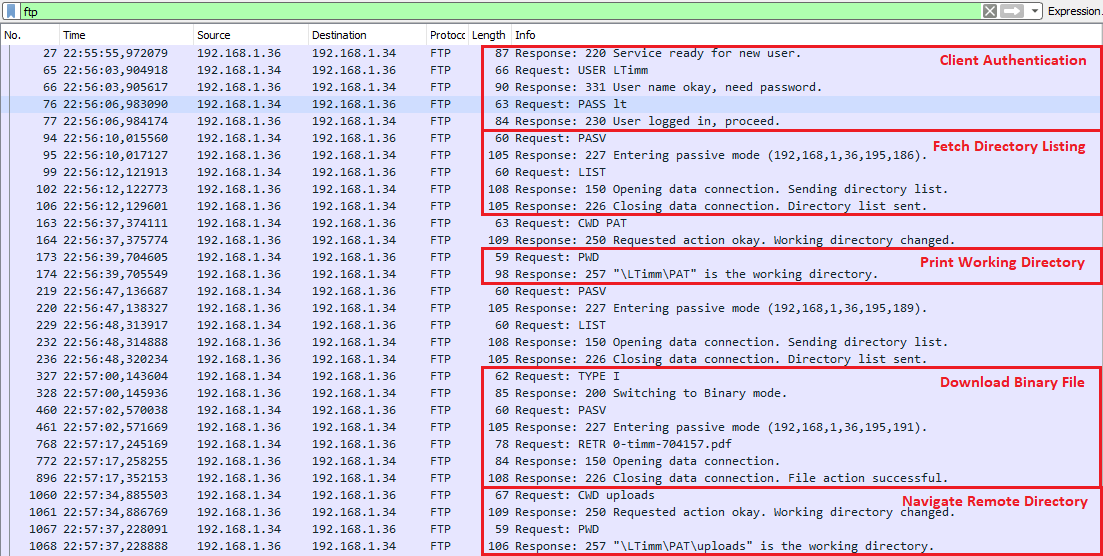
\includegraphics[width=0.9\columnwidth]{ClientServer1anno.png}
	\caption{blah blahr}
	\raggedright
	\label{fig:ourWS1}
\end{figure}

\begin{figure}[h]
	\centering
	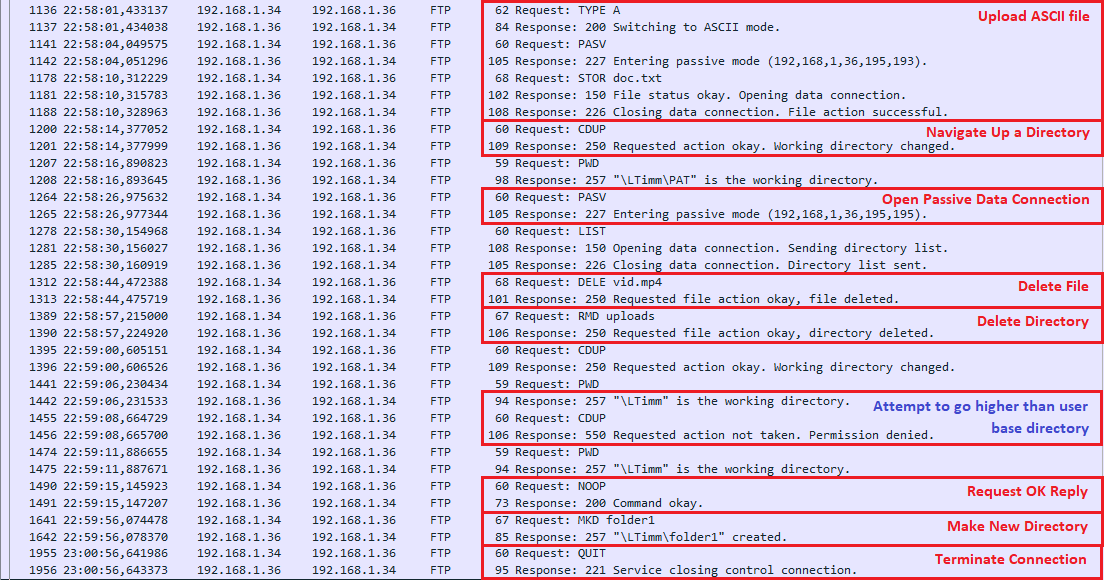
\includegraphics[width=0.9\columnwidth]{ClientServer2anno.png}
	\caption{blah}
	\raggedright
	\label{fig:ourWS2}
\end{figure}

\begin{figure}[h]
	\centering
	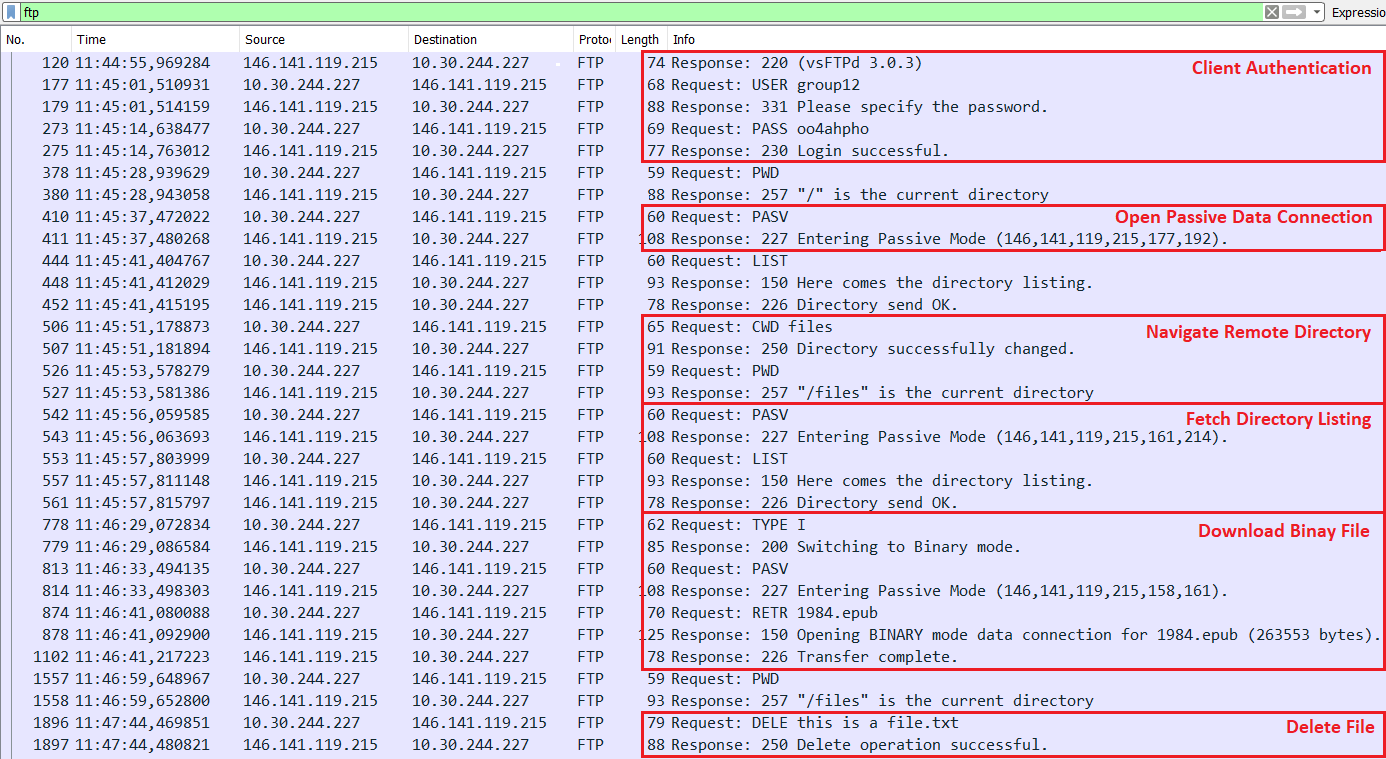
\includegraphics[width=0.9\columnwidth]{WitsCaptureAnno2.png}
	\caption{Wireshark screenshot 1 of functionality testing with standard FTP server}
	\raggedright
	\label{fig:WitsWS1}
\end{figure}

\begin{figure}[h]
\centering
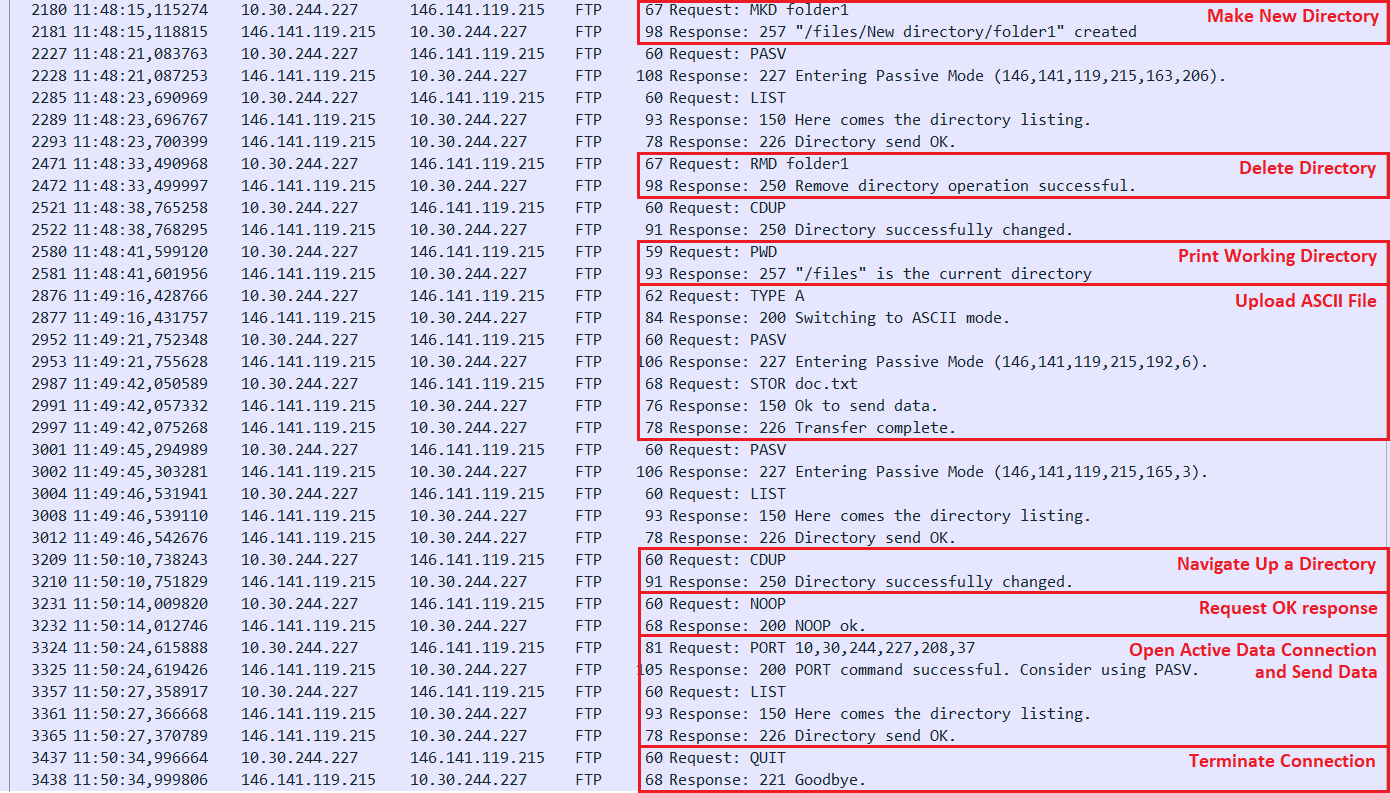
\includegraphics[width=0.9\columnwidth]{WitsServerCapture2.png}
\caption{Wireshark screenshot 2 of functionality testing with standard FTP server}
\raggedright
\label{fig:WitsWS2}
\end{figure}



\end{appendix}

%{\tiny \vfill \hfill \today \hspace{5mm} witseie-paper-2003.\TeX}


\end{document}

" vim: ts=4
" vim: tw=78
" vim: autoindent
" vim: shiftwidth=4
